\documentclass[twoside,10pt]{article}
\usepackage{/Users/bradenhoagland/latex/styles/toggles}
%\toggletrue{sectionbreaks}
%\toggletrue{sectionheaders}
\newcommand{\docTitle}{Percolation Processes on Dynamically Grown Graphs}
\usepackage{/Users/bradenhoagland/latex/styles/common}
\importStyles{formal}{rainbow}{plain}

%\renewcommand{\theenumi}{\alph{enumi}}

\usepackage{subfigure}

\usepackage[
        backend=biber,
]{biblatex}
\addbibresource{bib.bib}

%--------------------------------------------------------------------------------
% Custom commands
%--------------------------------------------------------------------------------
\newcommand{\poisson}{\text{Poisson}}
\newcommand{\BF}{Bohman-Frieze\xspace}

\begin{document}
%\tableofcontents

\title{Duke PRUV Research Project}{Braden Hoagland \quad\&\quad Rick Durrett}
\header{Braden Hoagland}{Dynamic Percolation Processes}

\warn{change std induced order map to be order of $\ang{1}_{\phi}$.}

\begin{abstract}
	We develop the theory of cluster growth near criticality for a general class of rules for dynamically growing graphs called two-choice rules. We use scaling theory to compute critical exponents for any two-choice rule, and we show special cases in which we can solve for these exponents explicitly. Finally, we consider the \ER rule, the simplest two-choice rule for which more explicit calculations are possible. We derive several of its important properties, then show that a large subset of two-choice rules - bounded size rules - behave like \ER near criticality.
\end{abstract}

%--------------------------------------------------------------------------------
% Introduction
%--------------------------------------------------------------------------------
\section{Introduction}

We begin with an empty graph on $n$ vertices, and at each step we add one edge chosen at random. If each step corresponds to time $1/n$, then as $n\to \infty$ the graph at time $t$ converges to an \ER graph in which the connection probability between any two edges is $2t/n$. A basic result on \ER graphs \cite{ER} is that there is a critical time $t_{c}=1/2$ at which point a giant component with order $n$ points emerges, which is referred to as ``percolation".

\begin{figure}[H]
	\centering
	\begin{subfigure}
		\centering
		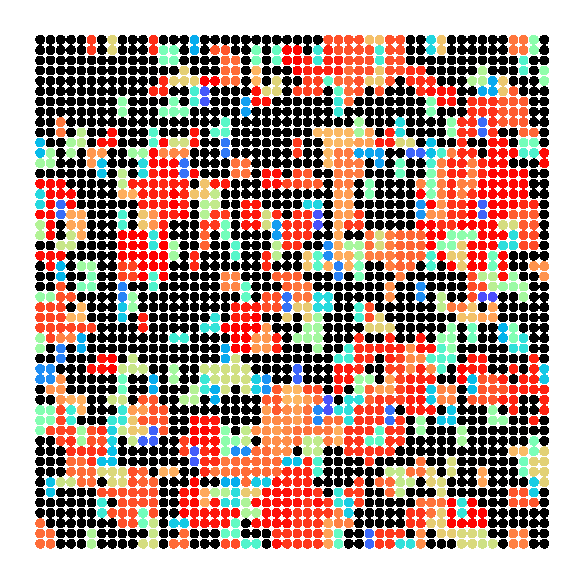
\includegraphics[scale=0.45]{fig/precrit.pdf}
	\end{subfigure}
	\begin{subfigure}
		\centering
		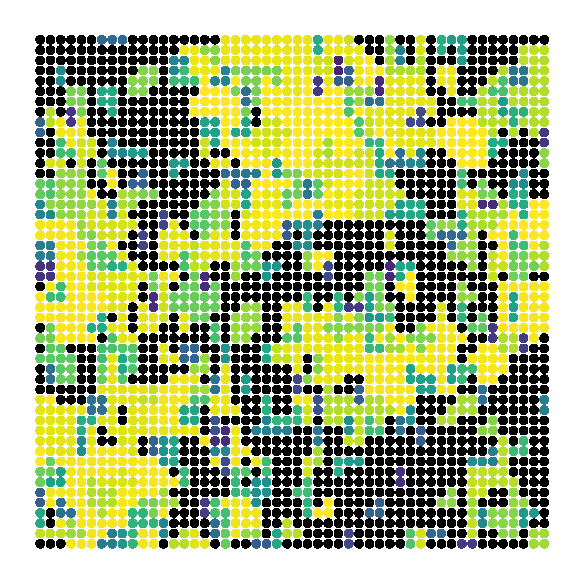
\includegraphics[scale=0.45]{fig/crit.pdf}
	\end{subfigure}
	\begin{subfigure}
		\centering
                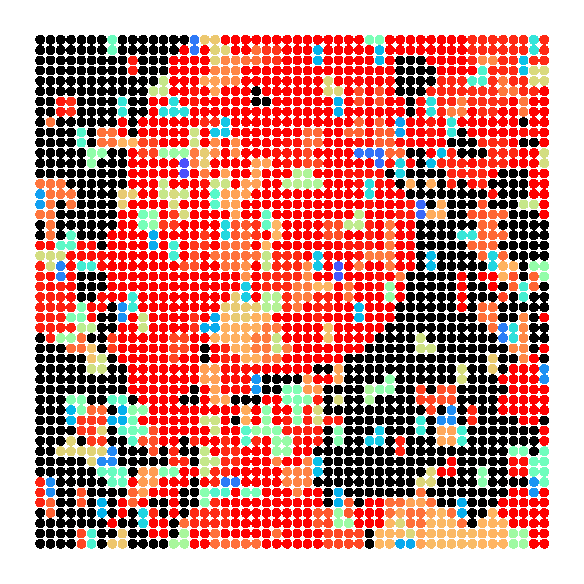
\includegraphics[scale=0.45]{fig/postcrit.pdf}
        \end{subfigure}
	\caption{The above is an approximation of the \ER process using 2500 vertices at times $t = \frac{2}{5} ,\frac{1}{2} ,$ and $\frac{3}{5} $, respectively. Black vertices are isolated; otherwise, vertices of the same color belong to the same cluster. Cluster color corresponds to cluster size, with blue clusters being small and red clusters large. Note that after time $\frac{1}{2} $, a single cluster has begun to dominate the graph.}
\end{figure}

The properties of the \ER model are well understood, so it serves as a natural reference point when studying other models. For example, if $\theta(t)$ is the fraction of vertices in the giant component (after we have let $n\to \infty$), then $\theta(t)\to 0$ as $t\searrow t_{c}$. This shows that the phase transition is continuous. Additionally, $\theta(t) \sim (t-t_{c})^{\beta}$, where $\beta=1$. This gives us a ``critical exponent" $\beta$ that describes the behavior of the process near $t_{c}$.

It is then natural to ask which generalizations of \ER graphs also have these properties. At a Fields Institute workshop in 2000, Dmitris Achlioptas suggested a class of variants of the \ER model, now dubbed ``Achlioptas processes". One starts with an empty graph, and at each step two edges $(v_1,v_2)$ and $(v_3,v_4)$ are randomly chosen from the set of all possible edges. Only one of them is added to the graph, though, according to some rule that depends on the cluster sizes of the current graph.

In 2001, Bohman and Frieze were the first to describe an Achlioptas process that delayed percolation \cite{BF}. At each step, the first edge is added if both $v_1$ and $v_2$ were isolated vertices, and the second edge is added otherwise. They showed that there was a constant $c_0>0.535$ such that the largest component at time $c_0$ has size bounded by $(\log n)^{O(1)}$. This rule is an example of a ``bounded size rule", in which all components of size greater than some constant $K$ are treated the same.

If $\kappa_i$ is the cluster size of $v_{i}$, then two possible rules are the sum rule and product rule. In the sum rule, the first edge is added if $\kappa_1+\kappa_2 < \kappa_3+\kappa_4$, and the second edge is added otherwise. In the product rule, the first edge is added if $\kappa_1 \kappa_2 < \kappa_3 \kappa_4$, and the second edge is added otherwise. In 2009, Achlioptas, D'Souza, and Spencer \cite{discontinuous} used numerical experiments to claim that the product rule exhibited ``explosive percolation" by causing a discontinuous phase transition at the critical time; however, in 2010, da Costa, et al. \cite{dacosta2010} found that the product rule's phase transition was actually continuous by comparing it to a strictly more explosive rule with continuous phase transition; the da Costa rule with parameter $m$ selected two groups of $m$ vertices at random and joined the vertices from each group with the smallest cluster size. In 2011, Riordan and Warnke showed that results for the da Costa rule could be greatly generalized: the phase transition at criticality is continuous for all $\ell$-vertex rules \cite{RW-cont}, which are a generalization of Achlioptas processes.

\begin{figure}[H]
        \centering
        \begin{subfigure}
                \centering
                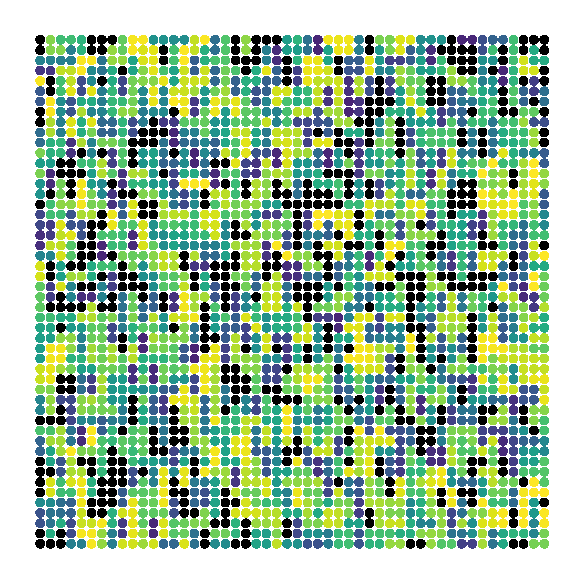
\includegraphics[scale=0.45]{fig/exp-precrit.pdf}
        \end{subfigure}
        \begin{subfigure}
                \centering
                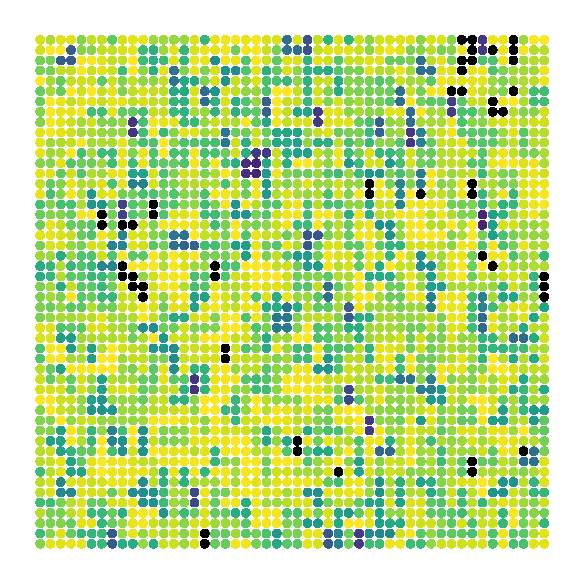
\includegraphics[scale=0.45]{fig/exp-crit.pdf}
        \end{subfigure}
        \begin{subfigure}
                \centering
                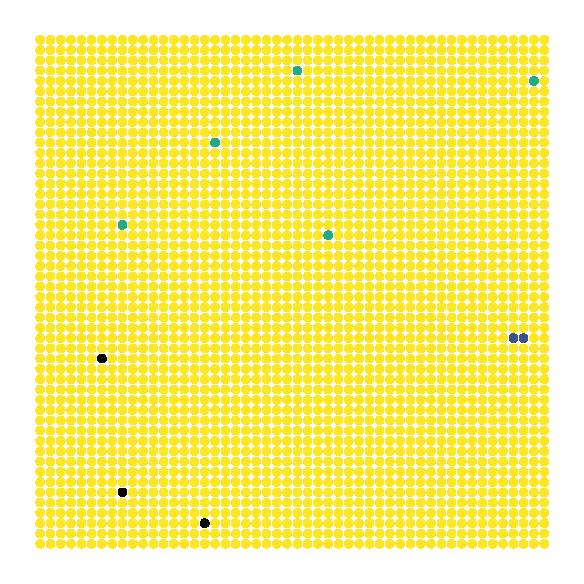
\includegraphics[scale=0.45]{fig/exp-postcrit.pdf}
        \end{subfigure}
	\caption{The above is an approximation of the da Costa rule with $m = 5$ at times $t = \frac{1}{2} ,\frac{3}{4} ,$ and $1$, respectively. Here we see explosive cluster growth: by time $\frac{3}{4} $, there are many large clusters cluttering the graph, and by time $t=1$, they have all merged into a single cluster that contains all but a handful of vertices.}
\end{figure}

In 2013, Bhamidi, Budhirja, and Wang showed that the behavior of the Bohman-Frieze process near the critical point was the same as in the \ER case \cite{coal}. Explicitly, they showed that at time $t_c + r/n^{1/3}$ for $-\infty<r<\infty$, the system converges to the ``multiplicative coalesent", in which clusters of size $x$ and $y$ merge at rate $xy$. Aldous had already showed a corresponding result for \ER graphs \cite{Aldous}, so this hinted at a deeper connection between the Bohman-Frieze and \ER processes. Through far from trivial, this result should not be surprising. After some time there will be very few isolated vertices, so the process will start to add edges \emph{almost} uniformly at random.

Then in 2017, Riordan and Warnke showed that \emph{all} bounded size Achlioptas processes share (in a strong sense) all the features of the \ER phase transition \cite{RW-bounded}. One unfortunate consequence of working in such generality is that Riordan and Warnke's work is largely based on contradiction, and thus it does not provide much quantitative information about the sizes of the graph clusters near criticality. Under the additional assumption of ``scaling behavior" that is supported by numerical evidence (see da Costa et al. \cite{daCosta}), though, it is possible to calculate further critical exponents for these processes.

The focus of this work will then be to generalize existing methods of calculating critical exponents, determining the classes of rules for which this is possible, and studying the limiting behavior of the critical exponents as their corresponding rules' parameters tend to extreme values.

%--------------------------------------------------------------------------------
% Two-Choice Rules
%--------------------------------------------------------------------------------
\section{Two-Choice Rules}

To begin, we will need to define some basic terms that will be used over and over again. Let $S$ be the fraction of vertices in the dominating cluster as $n \to \infty$. If $x_i$ is a vertex, then we denote its absolute cluster size by $\kappa_i$. Denote the probability that the minimum of $m$ independetly and randomly sampled vertices is $s$ by
\[
        Q_m(s, t) := \mathbb{P}\left( \min\left\{ \kappa_1, \dots, \kappa_m \right\} = s \text{ at time } t \right) .
\]
For notational simplicity we will drop the time $t$ from the notation. Consider the sum $\ang{1}_{m} := \sum_{s} Q_{m}(s)$, where the sum is over $x < \infty$. Since $S$ is the probability that a randomly chosen vertex belongs to an infinite cluster, we can write this sum as
\begin{equation}
	\ang{1}_{m} = \sum_{s} Q_{m}(s) = 1-S^{m}.
\end{equation}
Since $S=0$ for $t \leq t_{c}$ by definition, $\ang{1}_{m}=1$ for all $t \leq t_c$. Since they frequently show up in common examples, we give $m=1$ and $m=2$ shorthands:
\[
        P := Q_1, \quad\quad Q := Q_2.
\]
We also define
\[
	\ang{s^{k}}_{\phi} := \sum_{s} s^{k} \phi(s)
\] 
for any real-valued function $\phi$. In the special case $\phi = Q_{m}$, we will use the shorthand
\[
        \ang{s^{k}}_{m} := \ang{s^{k}}_{Q_{m}}.
\]
We will use $\Ang{\;\cdot\;}_{P}$ and $\ang{\;\cdot\;}_{Q}$ instead of $\Ang{\;\cdot\;}_{1}$ and $\ang{\;\cdot\;}_{2}$, respectively. Finally, we will use the notation $a(t) \sim b(t)$ to denote that $a(t)$ and $b(t)$ are asymptotically similar in the following sense: if $t$ approaches some critical value $t^{*}$ (which will be clear from context) such that $a(t), b(t) \to \infty$ as $t\to t^{*}$, then
\[
a(t) \sim b(t) \iff \frac{a(t)}{b(t)} \to C \text{ as } t\to t^{*}
\] for some nonzero constant $C$. It's straightforward to show that if $a(t) \sim b(t)$, then for any nonzero constants $\lambda, \mu$, we have $a(t) \sim \lambda a(t) \sim a(t) + \mu \sim b(t)$.

With these definitions in hand, we can turn our attention to the main results. We will be discussing rules that add a single edge every $t=1/n$ units of time, gotten by randomly sampling two groups of vertices independently from the graph, then choosing an endpoint vertex from each group. The following definition is a straightforward generalization of this idea, but we will only concern ourselves in this work with the case $\ell=2$.

\pagebreak

\begin{defn}[]
        Define a rule $\mathcal{R}$ as follows:
        \begin{itemize}
                \item Every $t=1/n$ units of time, choose $\ell$ groups of vertices $\mathcal{V}_1, \dots, \mathcal{V}_{\ell}$ (of potentially different sizes) by sampling vertices independent and at random from the graph.
                \item For each $i \in \left\{ 1, \dots, \ell \right\}$, follow some rule $\mathcal{F}_{i}$ to choose a vertex $x_i$ with cluster size $\kappa_i$ from group $\mathcal{V}_i$, subject to the condition that $\mathcal{F}_i$ induces a function $\phi_i(s) = \mathbb{P}\left( \kappa_i=s \right) $ that does not depend on any other $\phi_j$ for $j \neq i$.
        \end{itemize}
We call $\mathcal{R}$ an \textbf{$\ell$-choice rule}.
\end{defn}

If $\phi_{i}=Q_{m_i}$ for each $i$, then $\mathcal{R}$ is \textbf{minimizing}. We can similarly define \textbf{maximizing} rules. If each $\phi_i$ is the same, we say $\mathcal{R}$ is \textbf{symmetric}. We would like to restrict the vertex selection processes in each group as little as possible in order to get a more general theory, but for the concrete examples mentioned above, we can obtain more detailed results.

%-------------------
% The Scaling Assumption and Critical Exponents
%-------------------
\subsection{The Scaling Assumption and Critical Exponents}

Most of the results in this work follow from the assumption that near the critical time $t_c$, the function $P$ has the following form
\begin{equation}
	\label{scaling-assumption}
        P(s, t) = s^{1-\tau}f(s \delta^{1/\sigma}),
\end{equation}
where $\tau$ and $\sigma$ are constants, $f$ is a scaling function, $\delta:= t-t_{c}$, and $s$ is large. The following theorem gives relations between the exponents $\tau$ and $1/\sigma$ if some regularity conditions hold for the scaling function $f$.

\begin{thrm}
        \label{crit-exp}
        Suppose a rule $\mathcal{R}$ has a scaling function $f$ such that
        \begin{enumerate}
                \item $\lim_{x \to \infty} x^{2-\tau}f(x) = 0$; and
                \item $\int_{0}^{\infty} x^{2-\tau} f'(x) \;dx$ is finite.
        \end{enumerate}
        Then there are \textbf{critical exponents}
        \begin{align*}
                \beta &= (\tau-2)/\sigma, \\
                \gamma_{m} &= (m(2-\tau)+1)/\sigma.
        \end{align*}
        such that $S \sim \delta^{\beta}$ and $\ang{s^{k}}_{m} \sim \delta^{-\gamma_m-(k-1)/\sigma}$.
\end{thrm}
\begin{proof}
	We begin proving the first result. Since $S(t) = 1 - \sum_{s} P(s, t) = \sum_{s} ( P(s, t_c) - P(s, t))$, we can replace the sum with integration and substitute (\ref{scaling-assumption}) to get
        \begin{align*}
                S &\approx \int_{0}^{\infty} s^{1-\tau}(f(0)-f(s \delta^{1/\sigma})) \;ds.
                \intertext{We make the change of variable $s = x \delta^{-1/\sigma}$ to get}
                S &= \delta^{(\tau-2)/\sigma} \int_{0}^{\infty} x^{1-\tau} (f(0)-f(x)) \;dx.
                \intertext{Integrating by parts gives}
                S &= \frac{\delta^{(\tau-2)/\sigma}}{\tau-2} \left[ \left[ -x^{2-\tau} (f(0) - f(x)) \right]^{x=\infty}_{x=0} - \int_{0}^{\infty} x^{2-\tau} f'(x) \;dx \right].
        \end{align*}
        So by our assumptions on $f$, we have $S \sim \delta^{\beta}$, where $\beta = (\tau-2)/\sigma$. The derivation of $\gamma_{m}$ is similar.
\end{proof}

We will primarily be concerned with determining the critical exponents $1/\sigma, \tau$, and $\gamma_{m}$. More generally, we can also consider exponents $\gamma_{\phi}$ for any real-valued function $\phi$: $\gamma_{\phi}$ is the unique real number such that $\ang{s}_{\phi}\sim \delta^{-\gamma_{\phi}}$. By similar logic, we can see that for any $k$,
\begin{equation}
	\label{crit-exp-phi}
	\ang{s^{k}}_{\phi} \sim \delta^{-\gamma_{\phi}-(k-1)/\sigma}.
\end{equation}
As a consequence, we can determine $\gamma_{\phi}$ from $1/\sigma$ using any $k$. Thus we can always choose whichever one makes computations easiest.

%-------------------
% Induced Order Maps
%-------------------
\subsection{Induced Order Maps}

An important tool used throughout this work is the \emph{induced order map}, which encodes how quickly the giant component is growing at criticality. We use the term \emph{scaling form} to denote the function of $\delta$ that a particular value takes on as a result of the scaling assumption (\ref{scaling-assumption}). For example, the scaling form of $S$ is $\delta^{\beta}$, a direct result of \Cref{crit-exp}.

\begin{defn}[]
	Suppose $\zeta$ is a real-valued function of $S$, then the \textbf{induced order map} of $\zeta$ is the unique map $F_{\zeta}:\R\to \R$ such that $F_{\zeta}(\beta)$ gives the order of the scaling form of $\zeta(S)$. The \textbf{$i$-th standard induced order map} $F_{i}$ of an $\ell$-choice rule is the induced order map of $1 - \ang{1}_{\phi_{i}}$.
\end{defn}

\begin{ex}[]
Consider the map $f(S) = S^{a}$ for some constant $a$. In scaling form, $f(S) \sim \delta^{a \beta}$, so the induced order map $F_{f}$ is multiplication by $a$. Alternatively, consider the map $g(S) = b S$ for some constant $b$. In scaling form, $g(S) \sim b \delta^{a}$, so the induced order map $F_{g}$ is the identity. This is expected, as $g$ does not change the asymptotic behavior of the growth of $S$.
\end{ex}

\begin{ex}[]
	Consider the two-choice rule with $\phi_1 = \phi_2 = Q_{m}$. Both standard induced order maps are the same: the unique map $F$ such that $F(\beta)$ is the order of the scaling form of $1 - \ang{1}_{m}$. Recall the identity $1-\ang{1}_{m}= S^{m}$, which means the scaling form is $\delta^{m \beta}$, so $F(\beta) = m\beta$. Note that $F(\beta)=\beta$ for the \ER rule ($m=1$), i.e. $1 - \ang{1}_{P} = S \sim \delta^{\beta}$.
\end{ex}

We will see later on that the quantity $1-\ang{1}_{\phi}$ occurs quite naturally when describing the growth of the giant component near criticality, which motivates why we use it to define the standard induced order map. On a different note, the following theorem ties together critical exponents and induced order maps, allowing us to translate between the two whenever necessary.

\begin{prop}
	\label{exponent-to-induced-map}
	For any two-choice rule $\mathcal{R}$,
	\[
		\gamma_{\phi_{i}} = \frac{1}{\sigma} - F_{i}(\beta),
	\] where $F_{i}$ is the $i$-th standard induced order map of $\mathcal{R}$.
\end{prop}
\begin{proof}
	$\gamma_{\phi_i}$ is defined to be the real number satisfying $\ang{s}_{\phi} \sim \delta^{-\gamma_{\phi_i}}$. But by \Cref{crit-exp-phi} and the definition of standard induced order maps, $\ang{1}_{\phi_{i}} \sim \delta^{-\gamma_{\phi_i}+1/\sigma} = \delta^{F_{i}(\beta)}$. Thus $\gamma_{\phi_i} = 1/\sigma - F_{i}(\beta)$.
\end{proof}

In the following sections, we will derive scaling relations for general two-choice rules in terms of standard induced order maps, then use these to analyze minimizing rules and several other examples.


%-------------------
% Scaling Relations
%-------------------
\subsection{Scaling Relations}

Suppose $\mathcal{R}$ is a general two-choice rule, then, since the two sets are chosen independently,
	\begin{equation}
		\label{smoluchowski}
                \p_{t}{P(s)} = s \sum_{u+v=s} \phi_1(u) \phi_2(v) - s \phi_1(s) - s\phi_2(s).
	\end{equation}
	The summation term represents two components merging into a new component of size $s$, and the last two terms each represent a component of size $s$ joining with another component (this also has an integral form, which we will use when it's convenient). We can use this to calculate the growth rate of the giant component, which allows us to prove an important computational theorem.

\begin{lem}
        \label{2c-sdelS}
        For any two-choice rule $\mathcal{R}$, the fraction of vertices in the giant component $S$ satisfies
	\[
		\p_{t}{S} = \ang{s}_{\phi_1}\left( 1-\ang{1}_{\phi_2} \right) + \ang{s}_{\phi_2}\left( 1-\ang{1}_{\phi_1} \right).
	\] 
\end{lem}
\begin{proof}
        Using the identity $\sum_s P(s) = 1-S$, we calculate
        \begin{align*}
                \p_{t}{S} &= - \sum_s \p_{t}{P(s)} \\
                          &= - \sum_s s \sum_{u+v=s}\phi_1(u)\phi_2(v) + \sum_s s \phi_1(s) \sum_s + s \phi_2(s) \\
                          &= - \sum_u \sum_v (u+v) \phi_1(u)\phi_2(v) + \ang{s}_{\phi_1} + \ang{s}_{\phi_2} \\
                          &= -\sum_{u}u \phi_1(u) \sum_{v} \phi_2(v) - \sum_{u}\phi_1(u)\sum_{v}v \phi_2(v) + \ang{s}_{\phi_1} + \ang{s}_{\phi_2} \\
                          &= -\ang{s}_{\phi_1}\ang{1}_{\phi_2} - \ang{1}_{\phi_1}\ang{s}_{\phi_2} + \ang{s}_{\phi_1}+\ang{s}_{\phi_2} \\
                          &= \ang{s}_{\phi_1}\left( 1-\ang{1}_{\phi_2} \right) + \ang{s}_{\phi_2}\left( 1-\ang{1}_{\phi_1} \right).
        \end{align*}
\end{proof}

\begin{thrm}
	\label{2c-same-order}
	For any two-choice rule $\mathcal{R}$, there are nonnegative functions $\zeta_1$ and $\zeta_2$ such that
	\[
		\p_{t}{S} = \ang{s}_{\phi_1}\zeta_2(S) + \ang{s}_{\phi_2}\zeta_1(S).
	\] 
	Furthermore, the two terms above have the same order $F_1(\beta) + F_2(\beta) - 1/\sigma$ when the expression is put into scaling form, where $F_{i}$ is the $i$-th standard induced order map of $\mathcal{R}$.
\end{thrm}
\begin{proof}
	By \Cref{2c-sdelS}, we know $\p_{t}{S} = \ang{s}_{\phi_1}\left( 1-\ang{1}_{\phi_2} \right) + \ang{s}_{\phi_2}\left( 1-\ang{1}_{\phi_1} \right)$. Now for both $i$, consider the probability $\zeta_i(S)$ that a vertex chosen from group $i$ belongs to an infinite cluster. This satisfies the relation $\ang{1}_{\phi_i} = 1-\zeta_i(S)$, which allows us to recover the desired form of $\p_{t}{S} $. Then by \Cref{exponent-to-induced-map}, both terms have order $F_1(\beta) + F_2(\beta) - 1/\sigma$.
\end{proof}

To determine scaling relations for two-choice rules, we will need one last result, a consequence of \Cref{2c-same-order}.

\begin{cor}
	\label{2c-sdel-sp}
	For any two-choice rule $\mathcal{R}$, the average cluster size $\ang{s}_{P}$ satisfies
\[
        \p_{t}{\ang{s}_{P}} = 2\ang{s}_{\phi_1}\ang{s}_{\phi_2} - \ang{s^2}_{\phi_1}\zeta_2(S) - \ang{s^2}_{\phi_2}\zeta_1(S),
\]
where $\zeta_1$ and $\zeta_2$ are the functions from \Cref{2c-same-order}.
\end{cor}
\begin{proof}
	Recall from the proof of \Cref{2c-same-order} that there are functions $\zeta_1$ and $\zeta_2$ satisfying the relation $\ang{1}_{\phi_i} = 1-\zeta_i(S)$. We can then explicitly compute $\p_{t}{\ang{s}_{P}} $.
        \begin{align*}
                \p_{t}{\ang{s}_{P}} &= \sum_s s \p_{t}{P(s)} \\
                                    &= \sum_s s^2 \sum_{u+v=s}\phi_1(u)\phi_2(v) - \sum_s s^2 \phi_1(s) - \sum_s s^2 \phi_2(s) \\
                                    &= \sum_{u}\sum_{v} (u+v)^2\phi_1(u) \phi_2(v) - \ang{s^2}_{\phi_1}-\ang{s^2}_{\phi_2} \\
                                    &= \ang{s^2}_{\phi_1}\ang{1}_{\phi_2} + 2\ang{s}_{\phi_1}\ang{s}_{\phi_2} + \ang{1}_{\phi_1}\ang{s^2}_{\phi_2}- \ang{s^2}_{\phi_1}-\ang{s^2}_{\phi_2} \\
                                    &= 2\ang{s}_{\phi_1}\ang{s}_{\phi_2} + \ang{s^2}_{\phi_1}(\ang{1}_{\phi_2} - 1) + \ang{s^2}_{\phi_2}(\ang{1}_{\phi_1}-1) \\
                                    &= 2\ang{s}_{\phi_1}\ang{s}_{\phi_2} - \ang{s^2}_{\phi_1}\zeta_2(S) - \ang{s^2}_{\phi_2}\zeta_1(S).
        \end{align*}
\end{proof}

\begin{thrm}[]
	\label{2c-scaling-relations}
	For any two-choice rule with standard induced order maps $F_{i}$,
	\begin{align*}
		\gamma_{\phi_1} &= F_2(\beta) - \beta + 1,\\
		\gamma_{\phi_2} &= F_1(\beta) - \beta + 1,\\
		\gamma_{P} &= F_1(\beta)+F_2(\beta) - 2\beta + 1,\\
		\frac{1}{\sigma} &= F_1(\beta) + F_2(\beta) - \beta + 1,\\
		\tau &= \frac{\beta}{F_1(\beta)+F_2(\beta)-\beta+1} +2.
	\end{align*}
\end{thrm}
\begin{proof}
	Since $\p_{t}{S} \sim \delta^{\beta-1}$, \Cref{2c-same-order} shows
\[
	\frac{1}{\sigma} = F_1(\beta) + F_2(\beta) - \beta + 1.
\]
	Since $\p_{t}{S} = \ang{s}_{\phi_1}\zeta_2(S) + \ang{s}_{\phi_2}\zeta_1(S)$, the two dominating terms near criticality give us the system
\[
        \beta -1 \quad=\quad -\gamma_{\phi_1} + F_2(\beta) \quad=\quad -\gamma_{\phi_2} + F_1(\beta).
\]
This system implies
\begin{align*}
        \gamma_{\phi_1} &= F_2(\beta) - \beta + 1,\\
        \gamma_{\phi_2} &= F_1(\beta) - \beta + 1.
\end{align*}
By \Cref{2c-sdel-sp}, we know $\p_{t}{\ang{s}_{P}} = 2\ang{s}_{\phi_1}\ang{s}_{\phi_2} - \ang{s^2}_{\phi_1}\zeta_2(S) - \ang{s^2}_{\phi_2}\zeta_1(S)$. The three terms in this expression all have order $F_1(\beta)+F_2(\beta) - 2/\sigma$, which gives the system
\[
        -\gamma_{P}-1 \quad=\quad -\gamma_{\phi_1}-\gamma_{\phi_2} \quad=\quad -\gamma_{\phi_1}-\frac{1}{\sigma} +F_2(\beta) \quad=\quad -\gamma_{\phi_2}-\frac{1}{\sigma} + F_1(\beta).
\]
Using our previously calculated expressions for $\gamma_{\phi_1}$ and $\gamma_{\phi_2}$ this system gives us
\[
        \gamma_{P} = F_1(\beta)+F_2(\beta) - 2\beta + 1.
\]
Finally, using the identity $\beta = (\tau-2)/\sigma$ from \Cref{crit-exp}, we get
\[
        \tau = \frac{\beta}{F_1(\beta)+F_2(\beta)-\beta+1} +2.
\]
\end{proof}

Suppose we are instead working with a minimizing two-choice rule, i.e. $\phi_1=Q_{a}$ and $\phi_2=Q_{b}$ for two positive integers $a$ and $b$. In this case, we have simpler forms for the scaling relations.

\begin{cor}
	\label{2c-minimizing-scaling-relations}
	For minimizing two-choice rules, the scaling relations from \Cref{2c-scaling-relations} become
\begin{align*}
        \gamma_{a} &= 1 + (b-1)\beta,\\
        \gamma_{b} &= 1+(a-1)\beta,\\
        \gamma_{P} &= 1+(a+b-2)\beta,\\
        \frac{1}{\sigma} &= 1+(a+b-1)\beta,\\
        \tau &= \frac{\beta}{1+(a+b-1)\beta} +2.
\end{align*}
\end{cor}
\begin{proof}
	The relation $\ang{1}_{m} = 1 - S^{m}$ holds for all $m$, so the induced order map for $Q_{m}$ is $\beta \mapsto m \beta$. The result then follows from \Cref{2c-scaling-relations}.
\end{proof}

\begin{ex}
	Da Costa et al. \cite{daCosta} studied the two-choice rule with $\phi_1=\phi_2=Q_{m}$ for some $m$. In this case, \Cref{2c-minimizing-scaling-relations} gives critical exponents
	\begin{align*}
		\gamma_{m} &= 1 + (m-1)\beta,\\
		\gamma_{P} &= 1 + (2m-2)\beta,\\
		\frac{1}{\sigma} &= 1 + (2m-1)\beta,\\
		\tau &= \frac{\beta}{1 + (2m-1)\beta} +2,
	\end{align*}
	which agree with those derived in \cite{daCosta}.
\end{ex}

%-------------------
% Limiting Behavior
%-------------------
\subsection{Limiting Behavior}

One might expect that as $a$ and $b$ grow, we can delay the emergence of the giant component since we have more control over which vertices are connected. The following proposition makes this notion precise in terms of induced order maps.

\begin{prop}
	\label{2c-limits}
	Suppose $\mathcal{R}$ is a two-choice rule with standard induced order maps $F_1$ and $F_2$. If $F_i(\beta)\to 0$ as $a,b\to \infty$ for both $i$, then the critical exponents for $\mathcal{R}$ have limits
	\[
		\gamma_{\phi_1} = \gamma_{\phi_2} = \gamma_{P} = \frac{1}{\sigma} = 1, \qquad \tau = 2.
	\]
\end{prop}
\begin{proof}
	Suppose $\mathcal{R}$ is a two-choice rule with induced order maps $F_1, F_2$, then by \Cref{2c-scaling-relations} its scaling relations are
\begin{align*}
	\gamma_{\phi_1} &= F_1(\beta)-\beta+1,\\
	\gamma_{\phi_2} &= F_1(\beta)-\beta+1,\\
	\gamma_{P} &= F_1(\beta)+F_2(\beta)-2\beta+1,\\
	\frac{1}{\sigma} &= F_1(\beta)+F_2(\beta)-\beta+1,\\
	\tau &= \frac{\beta}{F_1(\beta)+F_2(\beta)-\beta+1} +2.
\end{align*}
If $F_{i}(\beta)\to 0$, then $1 - \ang{1}_{\phi_i} \to 1$, meaning $\ang{1}_{\phi_i}\to 0$ for both $i$. Then by \Cref{2c-sdelS}, the growth rate of the giant component is $\p_{t}{} S = 0$. If $\beta \to r$ for any $r \in \R - \left\{ 0 \right\}$, then $\p_{t}{} S$ cannot converge to $0$, so $\beta \to 0$ necessarily. Then since $\beta \to 0$ and $F_{i}(\beta)\to 0$ for both $i$, the limits in the proposition are straightforward computations.
\end{proof}

Of course, not all rules will satisfy this condition, as not all rules attempt to delay the critical time in the first place. It is an interesting question to determine broad families of rules for which $F_{i}(\beta)\to 0$ for both $i$ as $a,b \to \infty$. We conjecture that this applies for all minimizing two-choice rules.

\begin{conj}
	\label{m-beta-0}
        Suppose $\mathcal{R}$ is a minimizing two-choice rule with group sizes $a$ and $b$. Then $a\beta \to 0$ and $b\beta\to 0$, i.e. the limits in \Cref{2c-limits} apply.
\end{conj}

%-------------------
% Cluster Size Variance
%-------------------
\subsection{Cluster Size Variance}

The variance of the cluster size (at a fixed time) is, by definition, $\var_i(s) = \ang{s^2}_{\phi_i} - \ang{s}^2_{\phi_i}$. For two-choice rules, we can use our scaling relations to put this solely in terms of $\beta$ and the induced order maps, at least near criticality.
\begin{align*}
        \var_1(s) &= \delta^{-[\gamma_{\phi_1} + 1/\sigma]} - \delta^{-2\gamma_{\phi_1}} \\
                  &= \delta^{-[F_1(\beta)+2F_2(\beta)-2\beta+2]} + \delta^{-[2F_2(\beta)-2\beta+2]}.
\end{align*}
Similarly,
\[
        \var_2(s) = \delta^{-[2F_1(\beta)+F_2(\beta)-2\beta+2]} + \delta^{-[2F_1(\beta)-2\beta+2]}.
\]
Then if $F_i(\beta) \geq 0$ for both $i$, this is dominated by the first term. So near $t_c$, we have
\begin{align*}
        \var_1(s) &\approx \delta^{-[F_1(\beta)+2F_2(\beta)-2\beta+2]}, \\
        \var_2(s) &\approx \delta^{-[2F_1(\beta)+F_2(\beta)-2\beta+2]}.
\end{align*}
If $F_{i}(\beta)\to 0$ for both $i$, then we get the asymptotic behavior $\var_i(s) \to \delta^{-2}$. If $F_{i}(\beta) \leq 0$ for either $i$, then a similar argument with more cases gives the same limit.

\begin{ex}[]
        If $\mathcal{R}$ is a minimizing two-choice rule, then $F_1(\beta) = a \beta$ and $F_2(\beta)=b \beta$. Then
        \begin{align*}
                \var_1(s) &= \delta^{(2-a-2b)\beta-2},\\
                \var_2(s) &= \delta^{(2-2a-b)\beta-2}.
        \end{align*}
        If \Cref{m-beta-0} is true, then $\var_i(s) \to \delta^{-2}$ for both $i$.
\end{ex}

We can consider what happens in the limit for certain rules. If $F_{i}(\beta)\to 0$ as for both $i$ as $a,b\to \infty$, then by the proof of \Cref{2c-limits}, $\beta\to 0$ as well. Then a simple computation yields
\[
	\var_{i}(s) = \delta^{-2}
\] for both $i$. Thus if \Cref{m-beta-0} holds, this is true for minimizing two-choice rules.

If a rule is simple enough, we need not consider a limiting case of it to determine the variance of its cluster size distribution. For example, we know the \ER rule has $\beta=1$ (see \Cref{finding-beta}) and $F_{i}(\beta) = \beta = 1$ for both $i$. Thus for this simple rule, we get $\var_{i}(s) = \delta^{-3}$ for both $i$.

%--------------------------------------------------------------------------------
% \ER
%--------------------------------------------------------------------------------
\section{\ER}

The \ER rule is the simplest of all the two-choice rules. For each group, simply pick one vertex at random to be the group representative. Thus an equivalent way of defining the \ER rule is to add one of the $\binom{n}{2}$ possible edges in the graph at random at each time step.

This rule also has strong connections with the usual \ER random graphs. In particular, we can view the graph created by the \ER rule at time $t/n$ (so $t$ edges have been added) as an \ER graph with connection probability $\frac{2t}{n(n-1)}$. Thus in addition to our scaling theory, we can apply the theory of \ER random graphs to study this rule. We will denote \ER random graphs on $n$ vertices and with connection probability $p_c$ as $G(n,p_{c})$.

Before deriving our first results, we should note that the \ER rule is both minimizing and symmetric, so plugging in $a=b=1$ into the scaling relations from \Cref{2c-minimizing-scaling-relations} gives
\begin{equation}
	\label{ER-crit-exp}
        \gamma_{P} = 1, \qquad \frac{1}{\sigma} = 1 + \beta, \qquad \tau = \frac{\beta}{1+\beta} +2.
\end{equation}
With such a simple rule, we can in fact determine much more. In particular, we can determine $\beta$, which in turn fixes the other critical exponents. We will show $\beta=1$ (see \Cref{beta1} below), which subsequently implies $\sigma = 1/2$ and $\tau = 5/2$.

%-------------------
% Finding $\beta$
%-------------------
\subsection{Finding \texorpdfstring{$\beta$}{beta} for \ER}
\label{finding-beta}

\begin{lem}
	For the \ER rule, the critical time is $1/2$.
\end{lem}
\begin{proof}
	This is a result of translating between the \ER rule and \ER random graphs. It is well known \cite{princeton} that percolation in \ER random graphs occurs when the connection probability is $1/(n-1)$, which corresponds to using the \ER rule up until time $1/2$ by our earlier discussion.
\end{proof}

Note that since the critical time for the \ER rule is $t_c = t/n = 1/2$, this corresponds to adding $t=n/2$ edges to the graph. To find $\beta$ then, we can apply the theory of branching processes to study how connected the static graphs $G(n,t/n)$ are for $t < n/2$, as branching processes arise quite naturally in them.

\begin{thrm}[]
	\label{beta1}
	For the \ER rule, $\beta=1$.
\end{thrm}
\begin{proof}
	Suppose $t<n/2$, i.e. we are in the subcritical regime, and consider the \ER random graph $G(n,t/n)$. This has connection probability proportional to $G(n, 2t/(n (n-1)))$ by a factor of $2/(n-1)$, so as $n\to \infty$, this corresponds is a slowed down version of the \ER rule with critical time $t_{c}=1$.

	Let $v$ be a randomly chosen vertex and let $Z_{m}$ be the number of vertices at distance $m$ from $v$. When $m=o(\log n)$, the cluster containing $x$ is a tree with high probability, which makes $Z_{m}$ into a branching process where each individual has a $\poisson(t)$ number of offspring.

	The generating function for this distribution is
	\begin{align*}
		\phi(z) &= \sum_{k=0}^{\infty} r_{k}z^{k} \\
			&= \sum_{k=0}^{\infty} \frac{t^{k} e^{-t}}{k!} z^{k} \\
			&= e^{-t(1-z)}.
	\end{align*}
	We care about this in the limit as $t\to n/2$ and as $n\to \infty$, so we can suppose $t>1$. A standard result on branching processes is when $t>1$, the probability that the process dies out is given by the smallest $z \in [0,1]$ such that $z = \phi(z)$. This means the probability that the process \textit{never} dies out is $\theta = 1-z$.

	Letting $\mu := \phi''(1)$ and $z=1-\theta$ and expanding $\phi(1-\theta)$ in power series near 1 gives
	\begin{align*}
		z &= \phi(z) \\
		1-\theta &= \phi(1-\theta) \\
		1-\theta &\approx 1-t\theta + \frac{\mu\theta^{2}}{2} \\
		\theta &\approx \frac{2}{\mu} (t-1).
	\end{align*}
	Thus $\theta \sim t-1$. But in this slowed down version of \ER, the critical time is 1, so this is in the form $\theta \sim \delta$. By definition, $\beta$ is the exponent such that $\theta \sim \delta^{\beta}$, so $\beta=1$.
\end{proof}

%-------------------
% The Scaling Window
%-------------------
\subsection{The Scaling Window}

A critical assumption of this work was the scaling assumption, and for \ER, we can find an explicit bound on the size of the \textit{scaling window}, the region where the scaling assumption is accurate.

\begin{thrm}[]
	\label{crit-window}
	If $s$ is the cluster size, then for \ER, the scaling assumption holds after $t_{c}$ when $\delta = \Theta(s^{-1/2})$. Thus in the limit as $s\to \infty$, the scaling assumption is accurate in the entire postcritical regime.
\end{thrm}
\begin{proof}
	We use the following two relationships, which \cite{daCosta} derives for symmetric minimizing two-choice rules when $t < t_c$ and $s$ is large.
\begin{itemize}
        \item $P(x) = \delta^{(\tau-1)/\sigma} \tilde{f}(x \delta^{1/\sigma})$;
        \item $\tilde{f}(x) \propto x^{\lambda} \exp\left( -Cx^{1 + \log_2 m} \right)$, where $\lambda = (1+\log_2 m)\left( 1 + \frac{1}{4m-2}  \right)-\frac{2m}{2m-1} $;
\end{itemize}
where $m$ is the group size. In the case of \ER, we know $m=1$, $\tau=5/2$, and $1/\sigma = 2$, so these reduce to
\[
        P(x) = \tilde{C} \delta^{2} x^{-1/2} \exp\left( -Cx \delta^{2} \right),
\]
where $ \tilde{C}$ is the constant of propotionality from $\tilde{f}$. To clean up notation, we use the shorthand $\mathcal{E}_x := \exp\left( -C x \delta^{2} \right)$. Also note that $\delta = t-t_c$ when $t > t_c$, so $\p_{t}{\delta} =1$. With these observations, we can begin the computation. When $s$ is large, \Cref{smoluchowski} becomes
\begin{align*}
        \p_{t}{P}(s) &= \frac{s}{2} \int_{0}^{s} P(u)P(s-u)\;du - sP(s) \\
        \p_{t}\left\{ \tilde{C} \delta^{2}s^{-1/2}\mathcal{E}_{s} \right\} &= \frac{s}{2} \int_{0}^{s} \tilde{C}^{2}\delta^{4}(su-u^2)^{-1/2} \mathcal{E}_{u}\mathcal{E}_{s-u} \; du \quad-\quad \tilde{C}\delta^{2}s^{1/2}\mathcal{E}_{s} \\
        \tilde{C} \delta \mathcal{E}_{s} \left[ 2s^{-1/2} - 2C\delta^{2}s^{1/2} \right] &= \tilde{C} \delta \mathcal{E}_{s} \left[ \frac{s}{2} \int_{0}^{s} \tilde{C}\delta^{3}(su-u^2)^{-1/2}  \; du \quad-\quad \delta s^{1/2} \right] \\
	2s^{-1/2} - 2C \delta^{2}s^{1/2} &= \frac{s}{2} \tilde{C} \delta^3 \int_{0}^{s} (su-u^2)^{-1/2}\;du \quad-\quad \delta s^{1/2}.
\end{align*}
	Consider the integral above. It's straightforward to check that $2\sin^{-1}(\sqrt{u/s} )$ is an antiderivative of $\frac{1}{\sqrt{su-u^2} } $ when $s$ is positive, so this integral evaluates to
	\begin{align*}
		\int_{0}^{s} \frac{1}{\sqrt{su-u^2} }\;du &= 2 \left( \sin^{-1}(1)-\sin^{-1}(0) \right) \\
							  &= \pi.
	\end{align*}
	Thus our ealier equation becomes
	\[
		2s^{-1/2} - 2C\delta^{2}s^{1/2} = \frac{1}{2} \tilde{C} \delta^{3} \pi s - \delta s^{1/2}.
	\]
        Note that the first term on the left hand side goes to zero as $s\to \infty$, so in the limit this becomes
	\[
		\left( \frac{1}{2} \tilde{C} \pi s \right)\delta^{2} + \left( 2C s^{1/2} \right)\delta - s^{1/2} =0.
	\]
	This quadratic has roots
	\[
	\delta = \frac{-2C s^{1/2} \pm \sqrt{4 C^2 s + 2 \tilde{C} \pi s^{3/2}} }{\tilde{C} \pi s}.
	\]
	The only valid root is the positive one since $\delta >0$ in the postcritical regime. This root is $\Theta(s^{-1/2})$ when $s$ is large.
\end{proof}

Thus for large clusters formed by the \ER rule, the scaling assumption is perfectly reasonable. We have been unable to extend this result to more complicated rules, although it is believed that the scaling assumption also holds in the general case.

\begin{figure}[H]
        \centering
        \begin{subfigure}
                \centering
                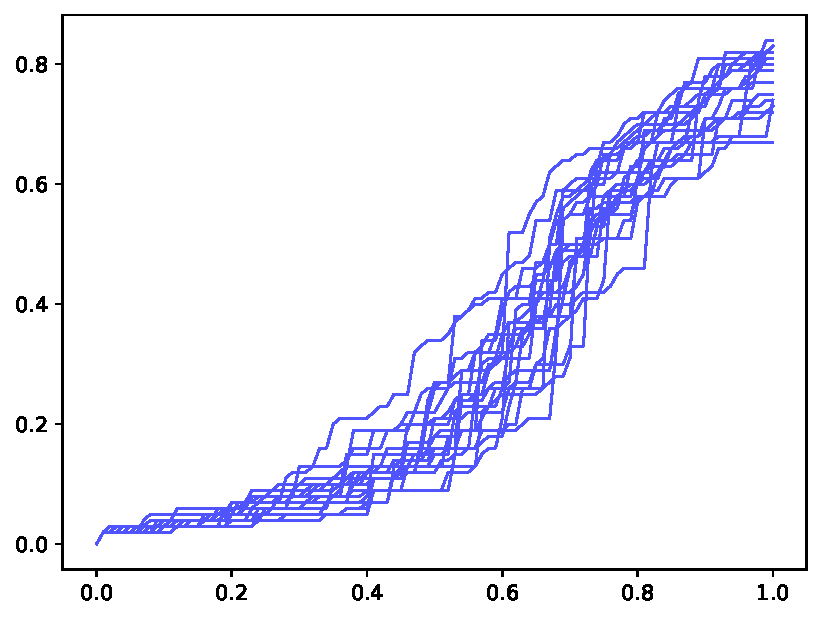
\includegraphics[scale=0.3]{fig/100.pdf}
        \end{subfigure}
        \begin{subfigure}
                \centering
                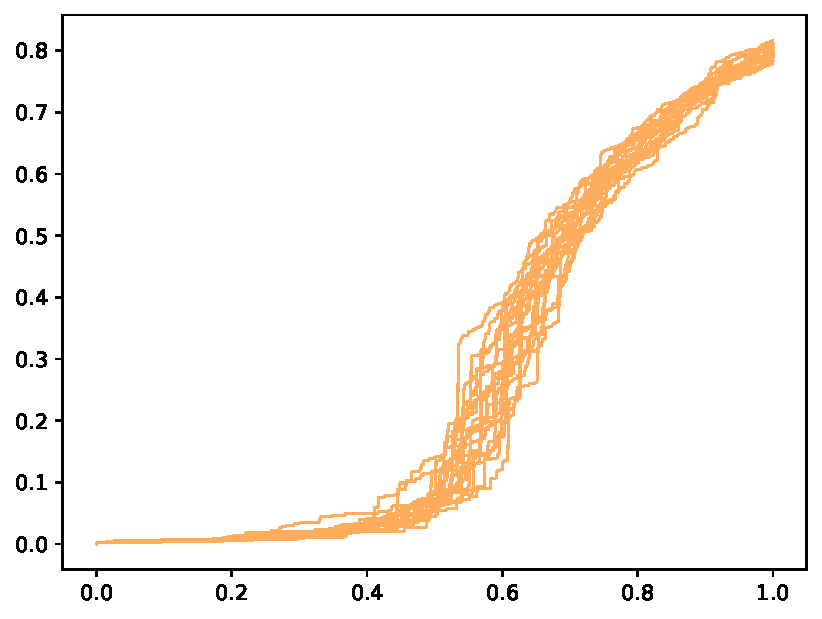
\includegraphics[scale=0.3]{fig/1000.pdf}
        \end{subfigure}
        \begin{subfigure}
                \centering
                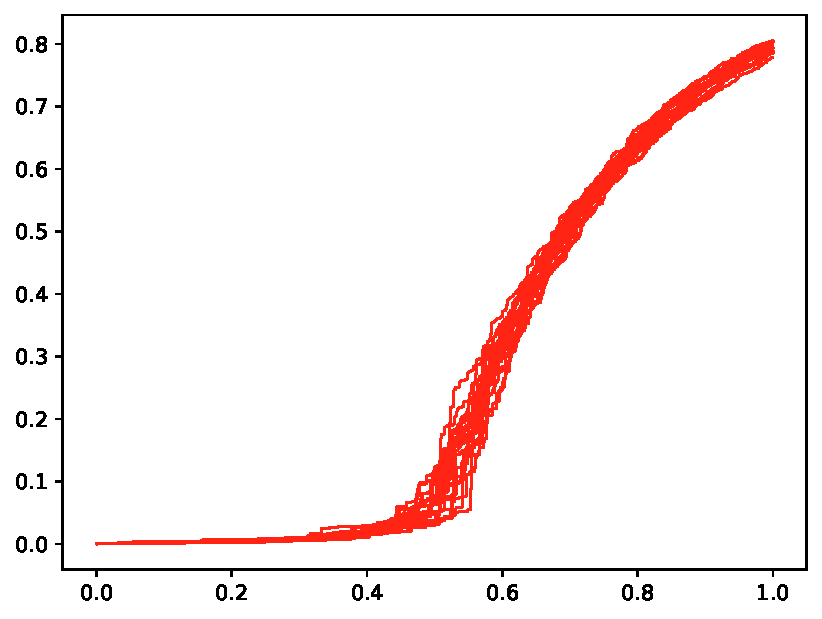
\includegraphics[scale=0.3]{fig/2500.pdf}
        \end{subfigure}
        \caption{The above plots show the fraction of vertices in the giant component for 20 \ER processes graphs with $n=100, 1000,$ and $2500$ vertices, respectively. The fact that $\beta=1$, i.e. $\theta \sim \delta$, means that the slopes of these lines at $t=1/2$ become linear in the limit as $n\to \infty$. Furthermore, \Cref{crit-window} implies that as $n\to \infty$, the entire plot after $t=1/2$ becomes linear.}
\end{figure}


%-------------------
% Bounded Size Rules
%-------------------
\subsection{Bounded Size Rules}

Since the \ER rule is so well understood, it is useful to know how any arbitrary rule relates to it. In particular, we can focus on rules that behave exactly like \ER, as characterized by critical exponents. These rules might have different subcritical and supercritical behavior, but as the giant component emerges, the rule produces similar graphs as \ER.

Bounded size rules are a very general category of rule that eventually start acting like \ER in the following sense: fix a constant $K \in \mathbb{N}$, then $\mathcal{R}$ is a bouded size rule if it treats all sampled vertices with $\kappa_i > K$ identically. In fact, \cite{RW-bounded} shows that bounded size rules share all the key features of \ER at criticality in a certain precise sense.

Intuitively, it makes sense that a bounded size rule eventually become similar to \ER. After enough clusters have been joined, the number of clusters of size $\leq K$ will be so small that it won't have much of an effect on the growth of the giant component. The key to noticing the complexity here is actually twofold:

\begin{enumerate}
	\item For any $k \leq K$, the number of clusters of size $k$ can be \textit{nonzero} at percolation (see \Cref{nonzero-at-criticality} below);
        \item After all clusters of size $\leq K$ have stopped having a real effect on the giant component, we're in a position much different than that of \ER. Instead of lots of isolated nodes, we have lots of finite size clusters.
\end{enumerate}

We can use a simple bounded size two-choice rule to examine these problems, which we do using a generalization of the well known \BF rule:
\begin{enumerate}
        \item At each step, pick $m$ vertices. These are the group 1 vertices.         \item If any of the $m$ vertices are isolated, pick the first such one as the group 1 representative. If not, sample one more random vertex and pick it no matter what.
        \item Repeat this for group 2, and connect the 2 group representatives with an edge.
\end{enumerate}
For this particular rule, we can explicitly track how the number of isolated clusters is changing through time; we will see that a nonzero proportion of our graph will be made up of isolated nodes at criticality.
\begin{prop}[]
	\label{nonzero-at-criticality}
	For the \BF rule with $m=1$, a nonzero proportion of the vertices in the graph are isolated at percolation.
\end{prop}
\begin{proof}
 We can explicitly write out the probability $\phi(s)$ that a representative's cluster size is $s$:
\[
        \phi(s)=
        \begin{cases}
                1 - (1-P_1)^{m+1} & s = 1, \\
                (1-P_1)^{m}P_s & s > 1.
        \end{cases}
\]
Let $m=1$, then \Cref{smoluchowski} gives
\begin{align*}
	\p_{t}{P_1} &= -2 \phi(1) \\
                    &= -2 + 2(1-P_1)^{m+1} \\
                    &= -2 + 2(1-P_1)^{2} \\
                    &= 2P_1^{2} - 4P_1.
\end{align*}
Solving this differential equation and using the initial condition $P_1(0)=1$ gives us the solution
\[
        P_1(t) = \frac{2}{e^{4t}+1} .
\]
We know that percolation occurs at $t=1$ at the very latest by \cite{RW-cont}. But plugging in $t=1$ gives $P_1(1) = \frac{2}{e^{4}+1} \approx 0.024$, so at criticality, a strictly positive proportion of our nodes are still isolated.
\end{proof}

As it turns out, this does not significantly affect cluster growth for bounded size rules, which we can formalize in terms of critical exponents (compare the following theorem with (\ref{ER-crit-exp})). This is a known result \cite{RW-bounded}, but using our theory of induced order maps, the proof is computational instead of by contradiction, as in \cite{RW-bounded}.

\begin{thrm}[]
Every bounded size two-choice rule has critical exponents
\[
	\gamma_{P}=1, \qquad \frac{1}{\sigma} =1+\beta, \qquad \tau = \frac{\beta}{1+\beta} +2.
\]
\end{thrm}
\begin{proof}
	Suppose we have a bounded size two-choice rule that treats all clusters of size $>K$ the same. Without loss of generality, suppose this rule is also symmetric with $\phi(s) = \P{ \kappa=s }$ (this argument really only applies to the representative selection process for one of the two vertex groups, so it readily extends to the case of non-symmetric rules). Finally, suppose each vertex group contains $m$ vertices.

	We'll also need a bit of new notation. Let $N \in \left\{ 0, \dots, m \right\}$ denote the number of vertices in our group whose cluster size is $\leq K$, and let $P_{\leq K} = P_1 + \cdots + P_{K}$. Then for $s>K$, we can partition $\phi(s)$ and use the fact that it acts exactly like \ER if all $m$ of the vertices in the group come from clusters of size $> K$.
	\begin{align*}
		\phi(s) &= \P{ \kappa = s \;|\; N = 0}\P{ N=0 } + \P{ \kappa = s \;|\; N>0 } \P{ N>0 } \\
			&= \frac{P_{s}}{S + \sum_{r>K}P_{r}} (1-P_{\leq K})^{m} + \P{ \kappa = s \;|\; N>0 } \P{ N>0 }.
	\end{align*}
	But $1-P_{\leq K} = S + \sum_{r>K}P_{r}$, so this becomes
	\[
		\phi(s) = P_{s}(1-P_{\leq K})^{m-1} + \P{ \kappa = s \;|\; N>0 } \P{ N>0 }.
	\]
	For $s \leq K$, we can use this same partition to get a similar expression.
	\begin{align*}
		\phi(s) &= \P{ \kappa = s \;|\; N = 0}\P{ N=0 } + \P{ \kappa = s \;|\; N>0 } \P{ N>0 } \\
			&= 0 + \P{ \kappa = s \;|\; N>0 } \P{ N>0 }.
	\end{align*}
	This allows us to sum over all $\phi(s)$ and thus calculate $\ang{1}_{\phi}$.
	\begin{align*}
		\sum_{s} \phi(s) &= \sum_{s > K} \phi(s) + \sum_{ s \leq K}\phi(s) \\
				 &= \left[ \sum_{s>K}(1-P_{\leq K})^{m-1} \right] + \left[ \sum_{s} \P{ \kappa=s\;|\; N>0 }\P{ N>0 } \right] \\
				 &= \Bigg[ (1-P_{\leq K})^{m-1}(1-S-P_{\leq K}) \Bigg] + \left[ (1-(1-P_{\leq K})^{m}) \sum_{s} \P{ \kappa=s\;|\; N>0 } \right] \\
				 &= (1- P_{\leq K})^{m-1} \left[ 1 - S - \xi + (\xi-1)P_{\leq K} \right] + \xi,
	\end{align*}
	where $\xi = \sum_{s} \P{ \kappa=s\;|\; N>0 }$. In scaling form, the first term above will be dominated by the \emph{smallest} critical exponent since $\delta$ is approaching 0. After multiplying everything out, the term with the lowest exponent will be $S$ (with critical exponent $\beta$).

	We will now induct on the group size $m$ to show that $\xi \sim 1$. When $m=1$,
	\[
	\sum_{s} \P{ \kappa=s\;|\; N>0 } = \sum_{s}\P{ \kappa=s\;|\; N=1 } = 1.
	\] Then assuming $\sum_{s} \P{ \kappa=s\;|\; N>0 } \sim 1$ when the group size is $m-1$,
	\begin{align*}
		\sum_{s}\P{ \kappa=s\;|\; N>0 } &= \sum_{s}\P{ \kappa=s\;|\; 0<N<m }\P{ 0<N<m\;|\;N>0 } \\
							 &\quad + \sum_{s} \P{ \kappa=s\;|\; N=m }\P{ N=m\;|\;N>0 } \\
							 &= \P{ 0<N<m\;|\; N>0 } \sum_{s} \P{ \kappa=s\;|\; 0<N<m } \\
							 &\quad + \P{ N=m\;|\;N>0 }\sum_{s}\P{ \kappa=s\;|\; N=m }.
	\end{align*}
	The first sum above is $\sim 1$ by our inductive hypothesis, and the second sum is exactly equal to 1. Thus
	\[
		\sum_{s}\P{ \kappa=s\;|\; N>0 } \sim \P{ 0<N<m\;|\; N>0 } + \P{ N=m\;|\;N>0 } = 1,
	\]
	as desired. Thus the scaling form of $\ang{1}_{\phi}=\sum_{s}\phi(s)$ is
	\[
	\ang{1}_{\phi} \sim \delta^{\beta}.
	\] 
	By definition, this fixes the standard induced order map of this rule. 	Note that for \ER, $\ang{1}_{P} = S \sim \delta^{\beta}$ as well, so both rules share the same standard induced order map. Since our computation of the critical exponents of two-choice rules relied only this map, the desired result follows.
\end{proof}

A crucial relation used in the previous theorem was the fact that
\[
\xi = \sum_{s} \P{ \kappa=s\;|\; N>0 }
\] is dominated by other terms as we approach criticality. For certain bounded size two-choice rules, more can be said of this term. For example, the \BF rule is a bounded size rule with threshold $K=1$, and $\xi_{BF}= 1$ since it always prioritizes connecting isolated vertices. It is already intuitively clear that the \BF rule cannot prioritize isolated clusters (more generally, the clusters below its size threshold) any further, but this classification gives that statement rigorous meaning.


%--------------------------------------------------------------------------------
% bibliography
%--------------------------------------------------------------------------------
\printbibliography


\end{document}
